\documentclass[fleqn,10pt]{wlscirep}

\usepackage{graphicx}
\usepackage{grffile}
\usepackage{textcomp}

\newcommand{\secref}[1]{Section~\ref{sec:#1}}
\newcommand{\tabref}[1]{Table~\ref{tab:#1}}
\newcommand{\figref}[1]{Figure~\ref{fig:#1}}

\newcommand{\beginsupplement}{%
        \setcounter{table}{0}
        \renewcommand{\thetable}{S\arabic{table}}%
        \setcounter{figure}{0}
        \renewcommand{\thefigure}{S\arabic{figure}}%
     }

\newcommand{\textapprox}{\raisebox{0.5ex}{\texttildelow}}

\graphicspath{{./images/}}


\title{Non-Parametric Mixture Modeling for Subtyping Tumors and Identifying Robust Expression Signatures}

\author[1,*]{Jacob Pfeil}
\author[1]{Geoff Lyle}
\author[1]{Ioannis Anastopoulos}
\author[1]{Lauren Sanders}
\author[1]{Katrina Learned}
\author[1]{Ellen Kephart}
\author[1]{Ann Durbin}
\author[1]{Holly Beale}
\author[1]{Sofie Salama}
\author[1,2]{Ted Goldstein}
\author[1]{David Haussler}
\author[1]{Olena Morozova}
\affil[1]{University of California, Santa Cruz, Biomolecular Engineering, Santa Cruz, 95064, United States}
\affil[2]{University of California, San Francisco}

\affil[*]{jpfeil@ucsc.edu}

%\keywords{Keyword1, Keyword2, Keyword3}

% TODO
% Write results 
% - make figure showing a normally distributed gene expression distribution
% - make neuroblastoma MYCN distribution
% Write methods 
% Write discussion
% Write introduction

\begin{abstract}
Precision oncology is changing the way medicine is practiced by incorporating high-throughput genomic analyses and data analytics. The field has focused on genomic variants, but gene expression data is becoming an additional tool for clinicians to improve patient outcomes. Here, we discuss a novel computational approach for identifying gene expression subtypes that may be helpful for future drug development and risk stratification. We apply this approach to synthetic data as well as patient data from the Cancer Genome Atlas Project. \end{abstract}
\begin{document}

\flushbottom
\maketitle
% * <john.hammersley@gmail.com> 2015-02-09T12:07:31.197Z:
%
%  Click the title above to edit the author information and abstract
%
\thispagestyle{empty}


\section*{Introduction}

% Cancer is heterogeneous
Heterogeneity across cancer patients has been increasingly recognized as an important factor influencing patient outcomes and response to targeted therapies. Cancers have been organized into subtypes using histology and genetic variants, but these clinical subtypes do not capture the full picture for many tumors. This has been underscored by large cancer genome sequencing projects such as ICGC, TCGA, and TARGET which have identified a long tail of genetic alterations \cite{armenia2018long}. The mutations in the tail are not common but may share similar biological features. Systematic characterization of cancer subtypes will lead to improved risk stratification and identification of novel drug targets \cite{zhao2018molecular}.

Molecular characterization of tumors is becoming an integrated component of modern cancer therapy. Clinicians are starting to incorporate genetic tests like those provided by Foundation Medicine or the UCSF500 gene panel into clinical practice. Somatic variant detection has been the most developed analysis for genomic medicine initiatives, but gene expression analysis is a cost-effective assay for identifying clinically useful features including differential expression, gene fusion events, and expressed variants. Gene expression also provides a measure of tumor infiltrating immune cells and has been used to predict response to immunotherapies \cite{auslander2018robust}.

Cancer subtyping based on gene expression data traditionally requires two steps. The first step is to cluster patients using an unsupervised method like k-means or agglomerative hierarchical clustering. The number of clusters is not usually known, so a parameter search is performed and the best performing model is nominated. Parameter searches are computationally expensive and may converge onto a suboptimal parameterization. The second step is to build a supervised classifier based on the cluster labels. This approach does not model the uncertainty in the clustering which may lead to over-fitting and suboptimal performance in the classification step \cite{zhao2018molecular}. Ideally, the clustering and classification would be generated in a single model that could improve the clustering and identify new clusters as data became available.

Fortunately, Bayesian non-parametric approaches have been developed that learn the number of clusters from the data and can be configured in an online learning setting to improve with each new classification problem. Non-parametric Bayesian models have been applied to microarray data to identify differentially expressed genes and to generate gene expression signatures \cite{medvedovic2002bayesian,newton2004detecting}. These methods are built upon a statistical model known as the dirichlet process \cite{gelman2014bayesian}. The dirichlet process provides a mechanism for learning parameters for a model from the data so that they do not have to be specified beforehand. 

Here, we describe the hydra pipeline which is an online clustering pipeline used to identify gene expression subtypes for precision oncology initiatives. The hydra pipline is built upon the non-parametric variational Bayes library bnpy \cite{hughes2014bnpy} and incorporates the molecular signatures database \cite{liberzon2011molecular} and the cancer hallmark gene sets generated by Goldstein et al. (2017). We show the performance of the hydra pipeline to predict pathway activity using synthetic data. We then apply the approach to identify well characterized breast cancer carcinoma subtypes. Finally, we apply the immune subtyping abilities of the pipeline to the TCGA melanoma data and identify a signature that predicts response to checkpoint blockade therapies.

%%%%%%%%%%%%%%%%%%%%%%%%%%%%%%%%%%
% Figure describing hydra %
%%%%%%%%%%%%%%%%%%%%%%%%%%%%%%%%%%
\begin{figure}
	\centering
	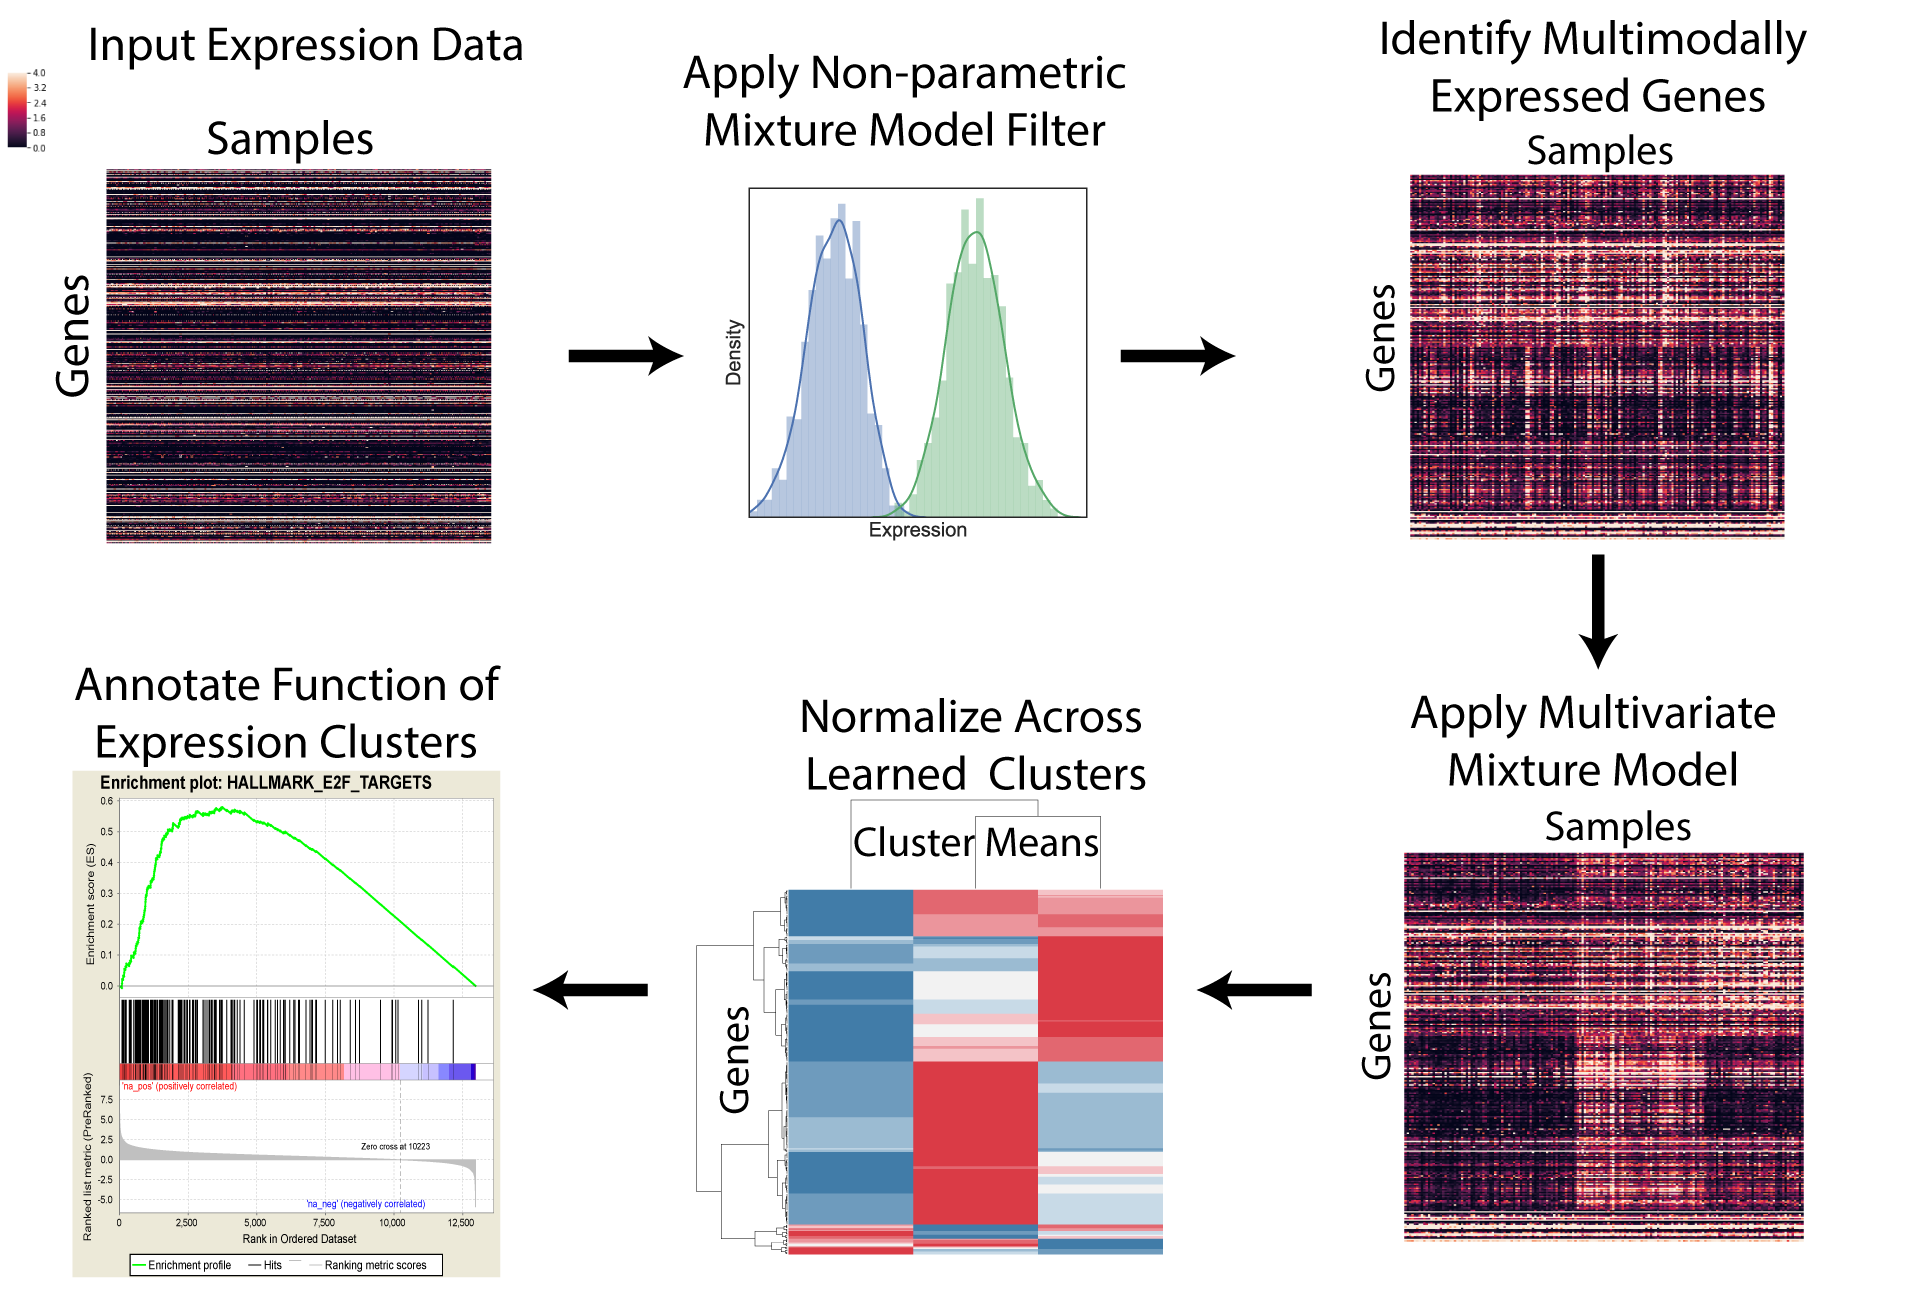
\includegraphics[width=0.75\linewidth]{images/hydra-overview@2x.png}
	\caption{Hydra Method Overview. The hydra pipeline works by taking an input matrix of gene expression profiles across an ideally homogeneous set of samples. The first step in the pipeline is to apply a non-parametric mixture model to learn differentially expressed genes. There is also an option to subset the genes of interest using curated gene sets. Once the multimodally expressed genes are identified, a multivariate mixture model is apply to learn the expression networks that can be used to subtype patients. The parameters are extracted and normalized and the normalized parameters are used to investigate the biological function of gene expression programs using gene set enrichment analysis.}
	\label{sfig:hydra-overview}
\end{figure}

\section*{Method Overview}
% Other approaches in the field
% Here I'll talke about the gene set enrichment approaches

% Overview of method
Hydra is built upon the Bayesian non-parametric python library bnpy \cite{hughes2014bnpy}. The benefit of a non-parametric approach is that the number of clusters does not need to specified because the algorithm is able to infer the number of clusters from the data. The bnpy library provides a flexible set of tools for performing Dirichlet process mixture modeling. Here, we use the Dirichlet process mixture modeling functions to identify multimodally expressed genes.

The input for the hydra approach is a genes by samples expression matrix. The first pass of the hydra pipeline is to identify all of the genes that are multimodally expressed and thus a potential biomarker. If a covariate is provided, then the hydra method will apply a Kruskal-Wallis test to determine if the difference in expression is dependent on the covariate \cite{mckight2010kruskal}. The goal of this analysis is to identify the genes that have a strong signal and may help to identify gene expression subtypes. The multimodally expressed genes are then assembled into a multivariate mixture modeling analysis to find gene expression signatures for subtyping tumors.

The output of the hydra pipeline includes the multimodally expressed genes, the training data, and the sample assignments. The bnpy model is also saved for future classification of patient tumors and can be used in an online learning setting where the model iteratively improves as data become available \cite{robert2014machine}. A jupyter notebook is also provided for preliminary cluster analysis that includes gene set enrichment analysis against the background expression \cite{kluyver2016jupyter,sergushichev2016algorithm}.

\section*{Results}

\subsection*{Synthetic Data Analysis}
% TODO: Add AUC table in supplemental
A synthetic data analysis was done to assess the performance of the hydra mixture modeling approach compared to rank-based approaches. The synthetic data was generated from GTEx skeletal muscle data and the MSigDB hallmark gene sets \cite{consortium2013genotype,liberzon2011molecular}. We used the 26 Hallmark gene sets with at least 100 genes. We randomly assigned a subset of the samples to have over-expression for each gene set. This process was repeated twice to created synthetic training and test data. We compared the hydra method to single sample gene set enrichment analysis (ssGSEA) \cite{barbie2009systematic} and gene set variation analysis (GSVA) \cite{hanzelmann2013gsva}. Both methods are implemented in the GSVA package. These methods are used widely in the field and have been used to identify biological pathway activation and subtype tumors.

Receiver operator curves were generated to visualize the performance of each method. Figure \ref{sfig:rocplot}A highlights two illustrative gene sets at two different effect sizes. The baseline expression for the Hallmark Glycoloysis gene set was lower than the Hallmark Oxidative Phosphorylation gene set, 2.28 and 2.83 log2(TPM + 1) respectively. We also compared the performance of these methods for two different effect sizes. One with a larger effect size of 1 and another with a smaller effect size 0.5 log2(TPM + 1).  

The hydra pipeline performed the best of the three methods. The hydra method performed best across the 26 Hallmark gene sets with a mean of AUC of 0.99 (95\% CI, 0.98 - 1.0 CI). ssGSEA method had a mean AUC of 0.93 (95\% CI, 0.90 - 0.96) followed by GSVA with a mean AUC of 0.85 (95\% CI, 0.82 - 0.89) \ref{sfig:rocplot}B). We found that the background expression for a gene set influenced the performance for ranking methods (Figure \ref{sfig:rocplot}C). Both the GSVA and ssGSEA AUC scores were negatively correlated with the background mean expression level with a Pearson correlation of -0.55 and -0.52, respectively. The hydra approach was not correlated with the background expression levels (p-value $>$ 0.05) \ref{sfig:rocplot}C).


%%%%%%%%%%%%%%%
% ROC Plot Figure %
%%%%%%%%%%%%%%%

\begin{figure}
	\centering
	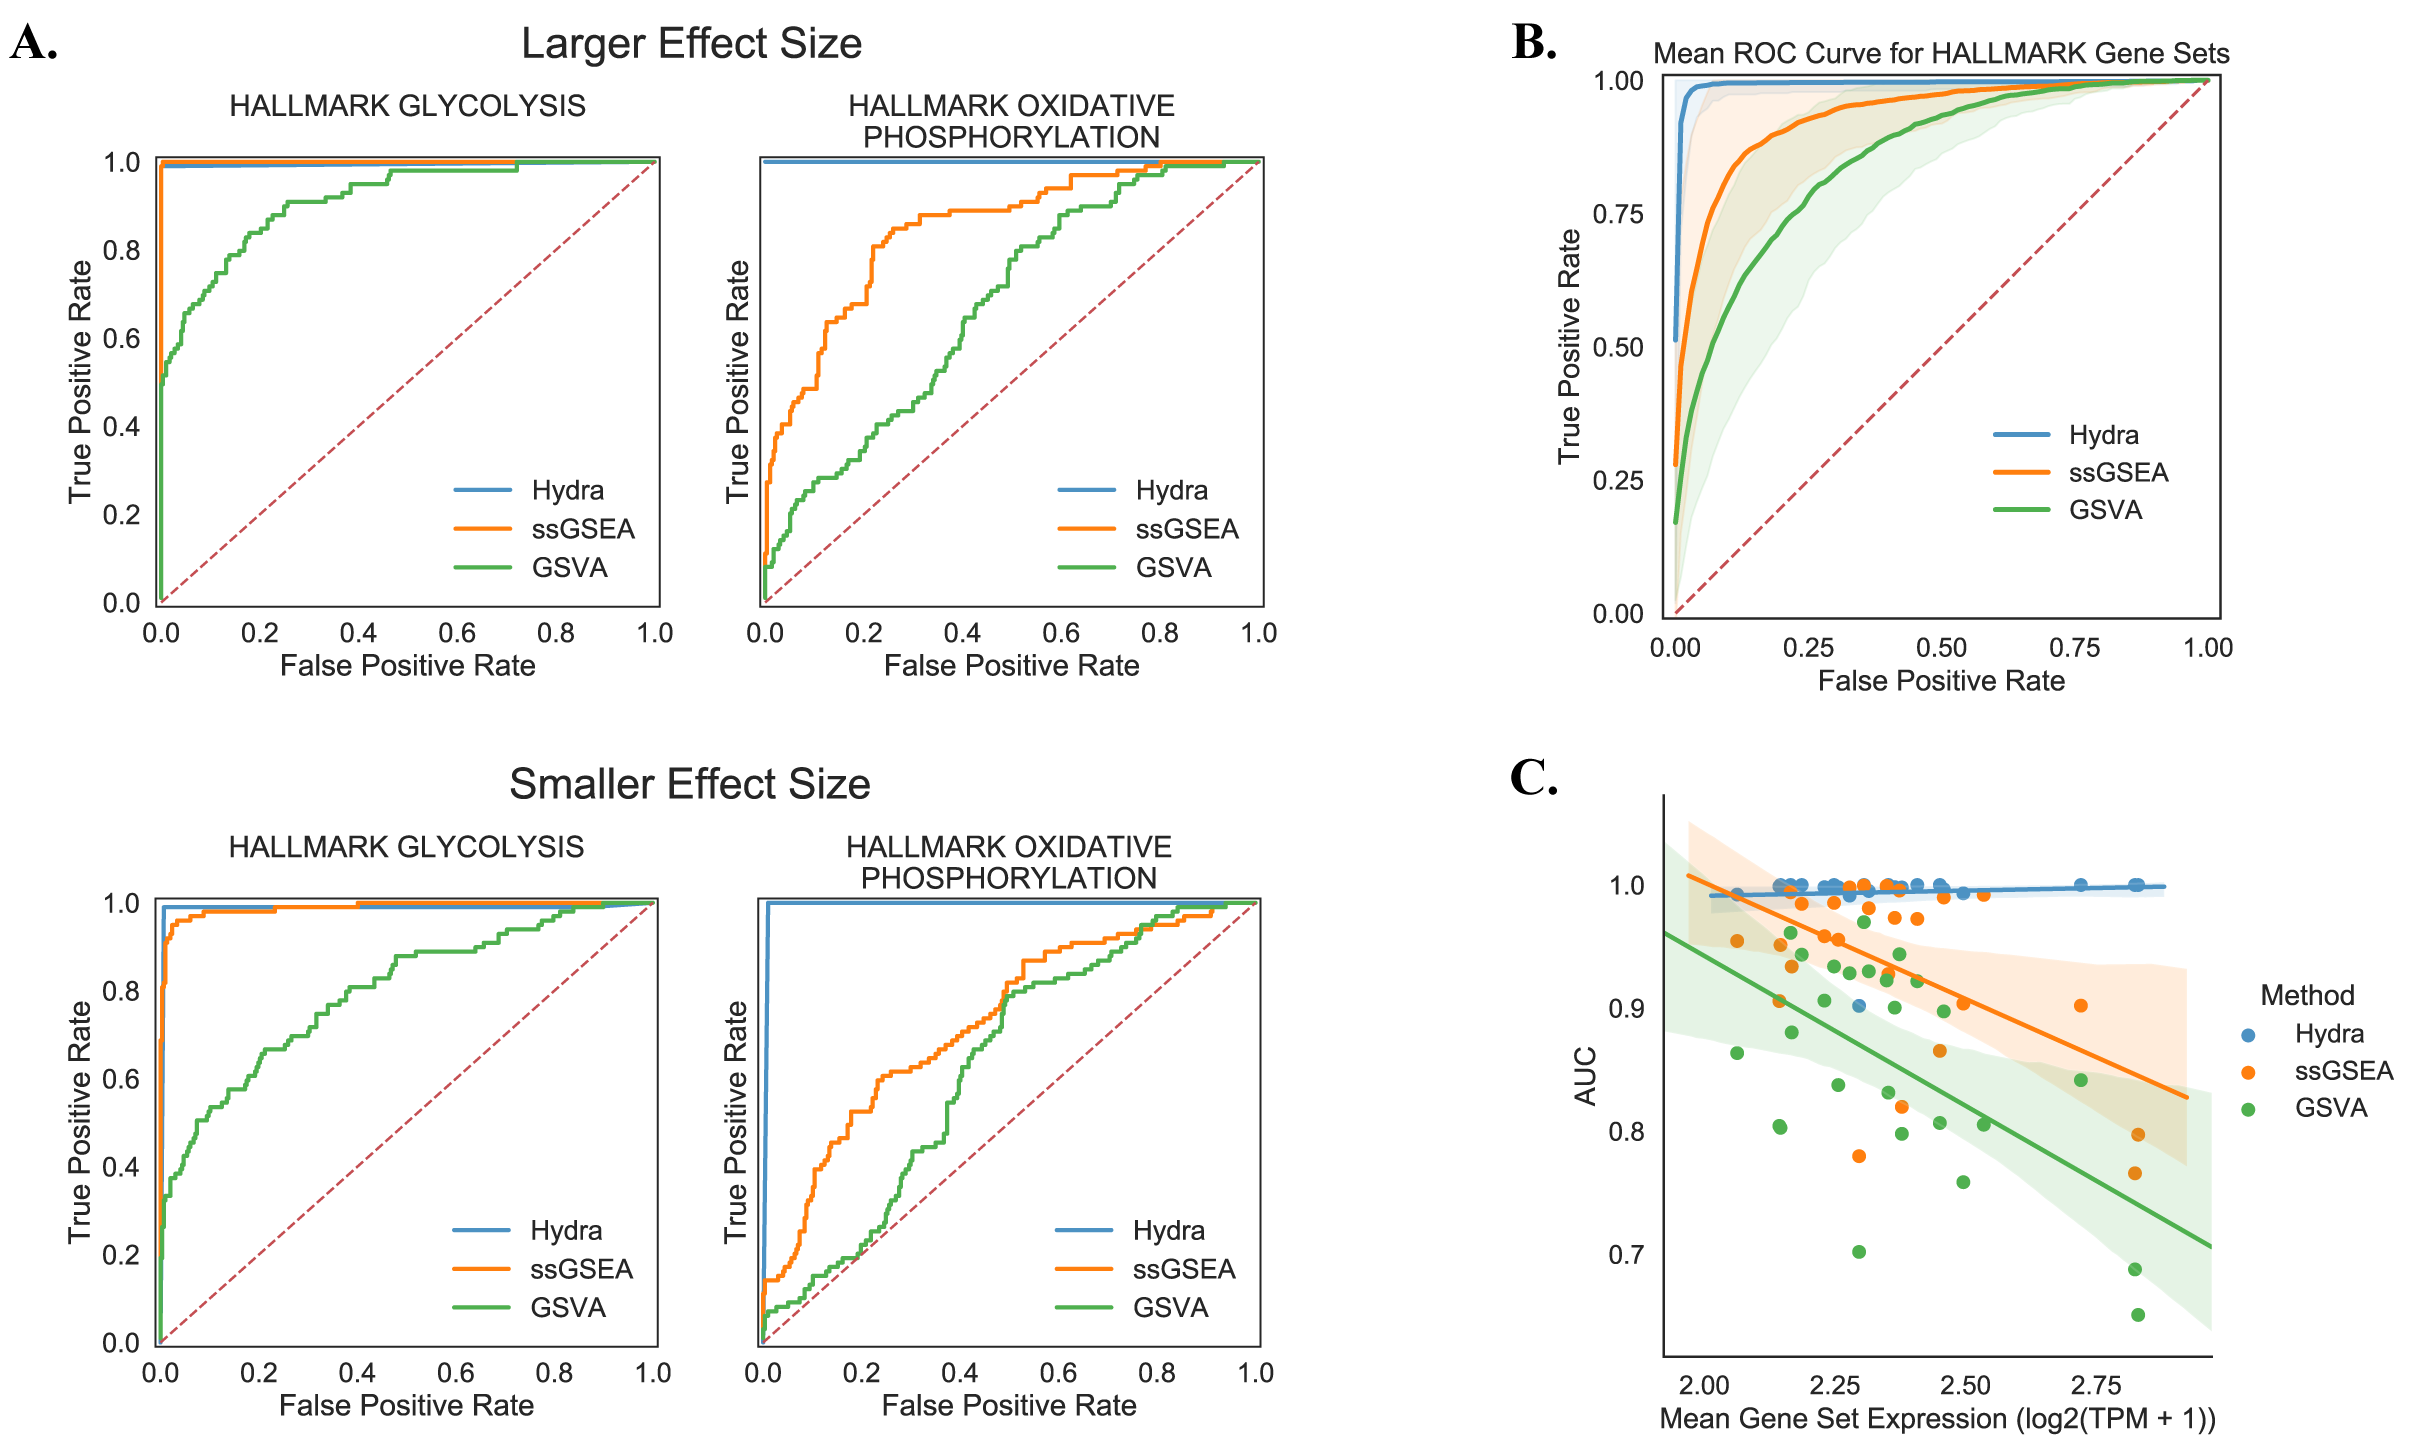
\includegraphics[width=0.8\linewidth]{images/figure-2-roc-curves@2x.png}
	\caption{Hydra is more sensitive than gene set enrichment approaches for detecting differential pathway activity in synthetic data. The performance of the ranking methods depends on the baseline expression for the gene set and the effect size (A). On average, the hydra approach performed the best across 26 simulated data sets using the HALLMARK gene sets. The performance of the rank-based methods was negatively correlated with the baseline expression for the gene set, but the hydra approach was not affected (C).}
	\label{sfig:rocplot}
\end{figure}

\subsection*{Immune Subtype Validation}
% TODO: Look into the general features of the differentially expressed genes
The tumor microenvironment plays an important role in providing nutrients and oxygen to the tumor, shielding cancer cells from the immune system, and providing growth factors that promote cancer growth and resistance to therapies \cite{hanahan2012accessories}. We applied the hydra method to identify immune subtypes of skin cutaneous melanoma from TCGA (N=469). The data was downloaded from the UCSC Xena browser \cite{vivian2017toil}.

We used the IMMPORT database of immune markers to narrow the set of genes for clustering to immune specific genes \cite{bhattacharya2018immport}. We removed any gene with a mean expression value less than 1 log2(TPM + 1). The hydra pipeline identified 253 differentially expressed genes out of the 1,740 genes in the IMMPORT database. Th 253 genes were used for the multivariate Gaussian mixture model analysis which identified 18 clusters (Figure \ref{sfig:melanoma}A). Hierarchical clustering across the cluster means identified 5 super-clusters (Figure \ref{sfig:melanoma}A). Clusters 0 and 1 were the most common with a posterior probability of ~13\% and clustered with low immune expression clusters. 

% TODO: Incude an estimate analysis as well
We next compared the leukocyte infiltrate fractions across hydra clusters. The leukocyte fraction was estimated by Saltz et al. (2018) using a convolutional neural network trained on H\&E stained slide images \cite{saltz2018spatial}. This analysis provides the total leukocyte fraction as well as estimates for specific immune cell populations using the CIBERSORT algorithm \cite{newman2015robust}. The clusters identified by the hydra pipeline had statistically different leukocyte fractions as well as lymphocyte, mast cell, dedritic cell, macrophage and eosinophil expression (Kruskal-Wallis test: p $<$ 0.01) (Figures \ref{sfig:melanoma}B and \ref{sfig:melanoma}C).

We then identified cluster specific features using gene set enrichment analysis \cite{subramanian2005gene,mootha2003pgc,sergushichev2016algorithm}. We pre-ranked a list of genes using the t-statistic generated by comparing the cluster specific expression levels to background expression of the disease population. Super cluster 1 not surprisingly showed high expression of T-cell and B-cell markers and markers of PD1 signaling, but each cluster also had specific immune associated expression patterns that differentiated them from their neighboring clusters. Super cluster 4 showed either a lack of immune associated expression or pathways associated with VPR interactions, MHC class II antigen presentation, or TGF-Beta signaling. 

Finally, we used the clustering pattern learned from the TCGA data to predict response to checkpoint blockade. We processed RNA-Seq data generated by Riaz et al. 2017 and used the N-of-1 classification scheme to label patient tumors by their TCGA cluster assignment. Our predictions found that partial and complete responders were more likely to be placed in super cluster 1 and progressive disease or stable disease patients were placed in super cluster 4.

%%%%%%%%%%%%%%%%%%%%%%%%%%%%%%
% SKCM Immune Subtype Figure %
%%%%%%%%%2%%%%%%%%%%%%%%%%%%%%%

\begin{figure}
	\centering
	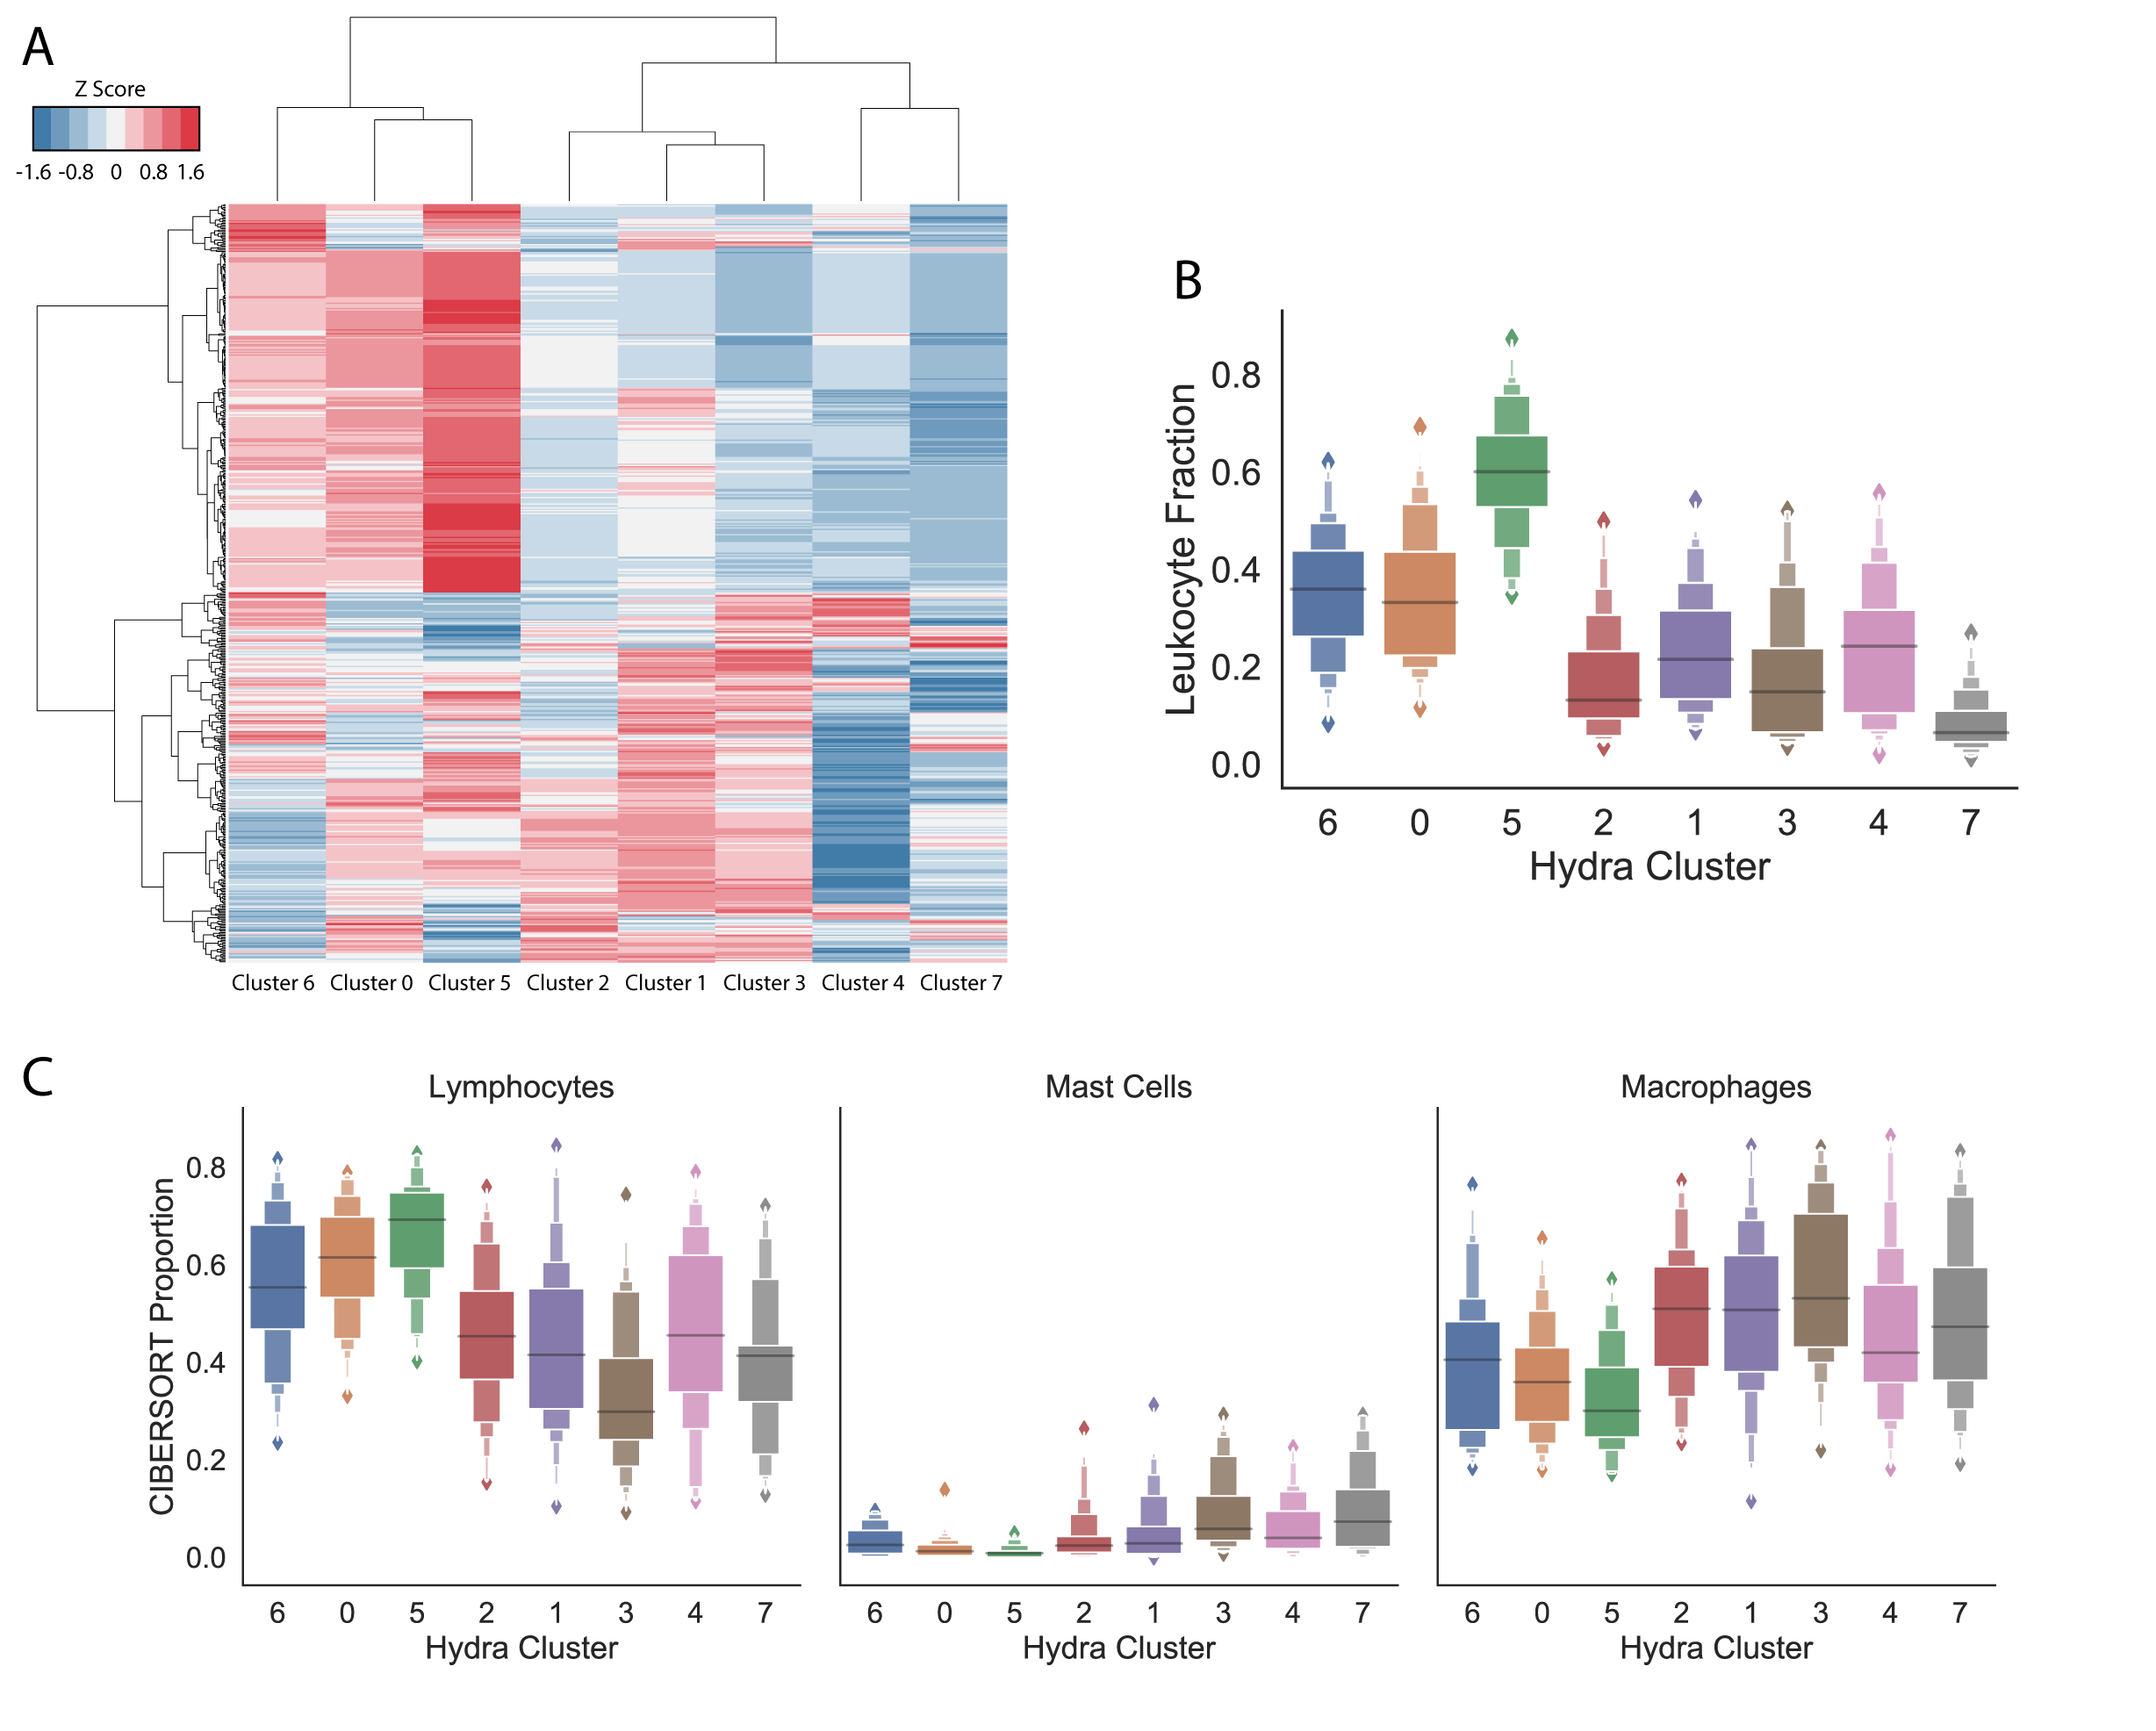
\includegraphics[width=0.75\linewidth]{images/melanoma-immune-subtypes-immport-boxen@2x.png}
	\caption{Melanoma Immune Subtyping and Validation. The hydra clustering algorithm identified 8 melanoma subtypes. Comparing these subtypes to a whole-slide image analysis of H\&E slides identified statistically significant differences in the leukocyte infiltrate across the hydra clusters (B). Further analysis of the clusters using the CIBSORT algorithm identified statistically significant differences for the lymphocyte, Mast cell, and macrophage expression (C). TODO: Make another figure where the immune cell expression is interspersed into one plot so show the contrast in immune infiltrate.}
	\label{sfig:melanoma}
\end{figure}

%%%%%%%%%%%%%%%%%%%%%%%%%%%%%%%
% SKCM Immune Survival Figure %
%%%%%%%%%2%%%%%%%%%%%%%%%%%%%%%

\begin{figure}
	\centering
	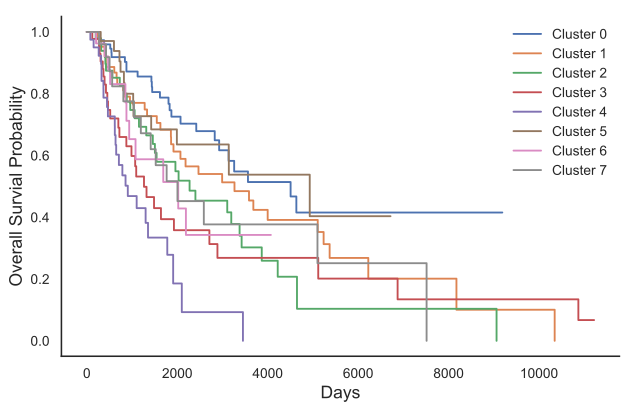
\includegraphics[width=0.75\linewidth]{images/immport-skcm-cluster-survival.png}
	\caption{Hydra Subtypes Predict Poor Survival in Melanoma.}
	\label{sfig:melanoma-surv}
\end{figure}


We next investigated the survival for different immune clusters and identified a survival benefit from a high lymphocyte to macrophage ratio. For example, cluster six grouped with the elevated lymphocyte fraction and had a statistically significant improvement in survival compared to a cluster that had lower immune infiltrate and a higher macrophage fraction (Figures \ref{sfig:melanoma} and \ref{sfig:melanoma-surv}). Gene set enrichment analysis for the subtypes that had a statistically significant survival benefit were also enriched for T-cell infiltrate whereas cluster 4 was not enriched for an immune gene set suggesting that the cancer cells were unchecked by the immune system . 

\subsection*{Molecular Subtype Validation}
Gene expression analysis is also used to identify molecular subtypes of cancer. Genetic and epigenetic alterations lead to changes in expression and these changes can be quantified using RNA-Seq technology and compared across patients to find molecular subtypes.


%%%%%%%%%%%%%%%%%%%%%%
% TCGA BRCA Subtypes %
%%%%%%%%%%%%%%%%%%%%%%
\begin{figure}
	\centering
	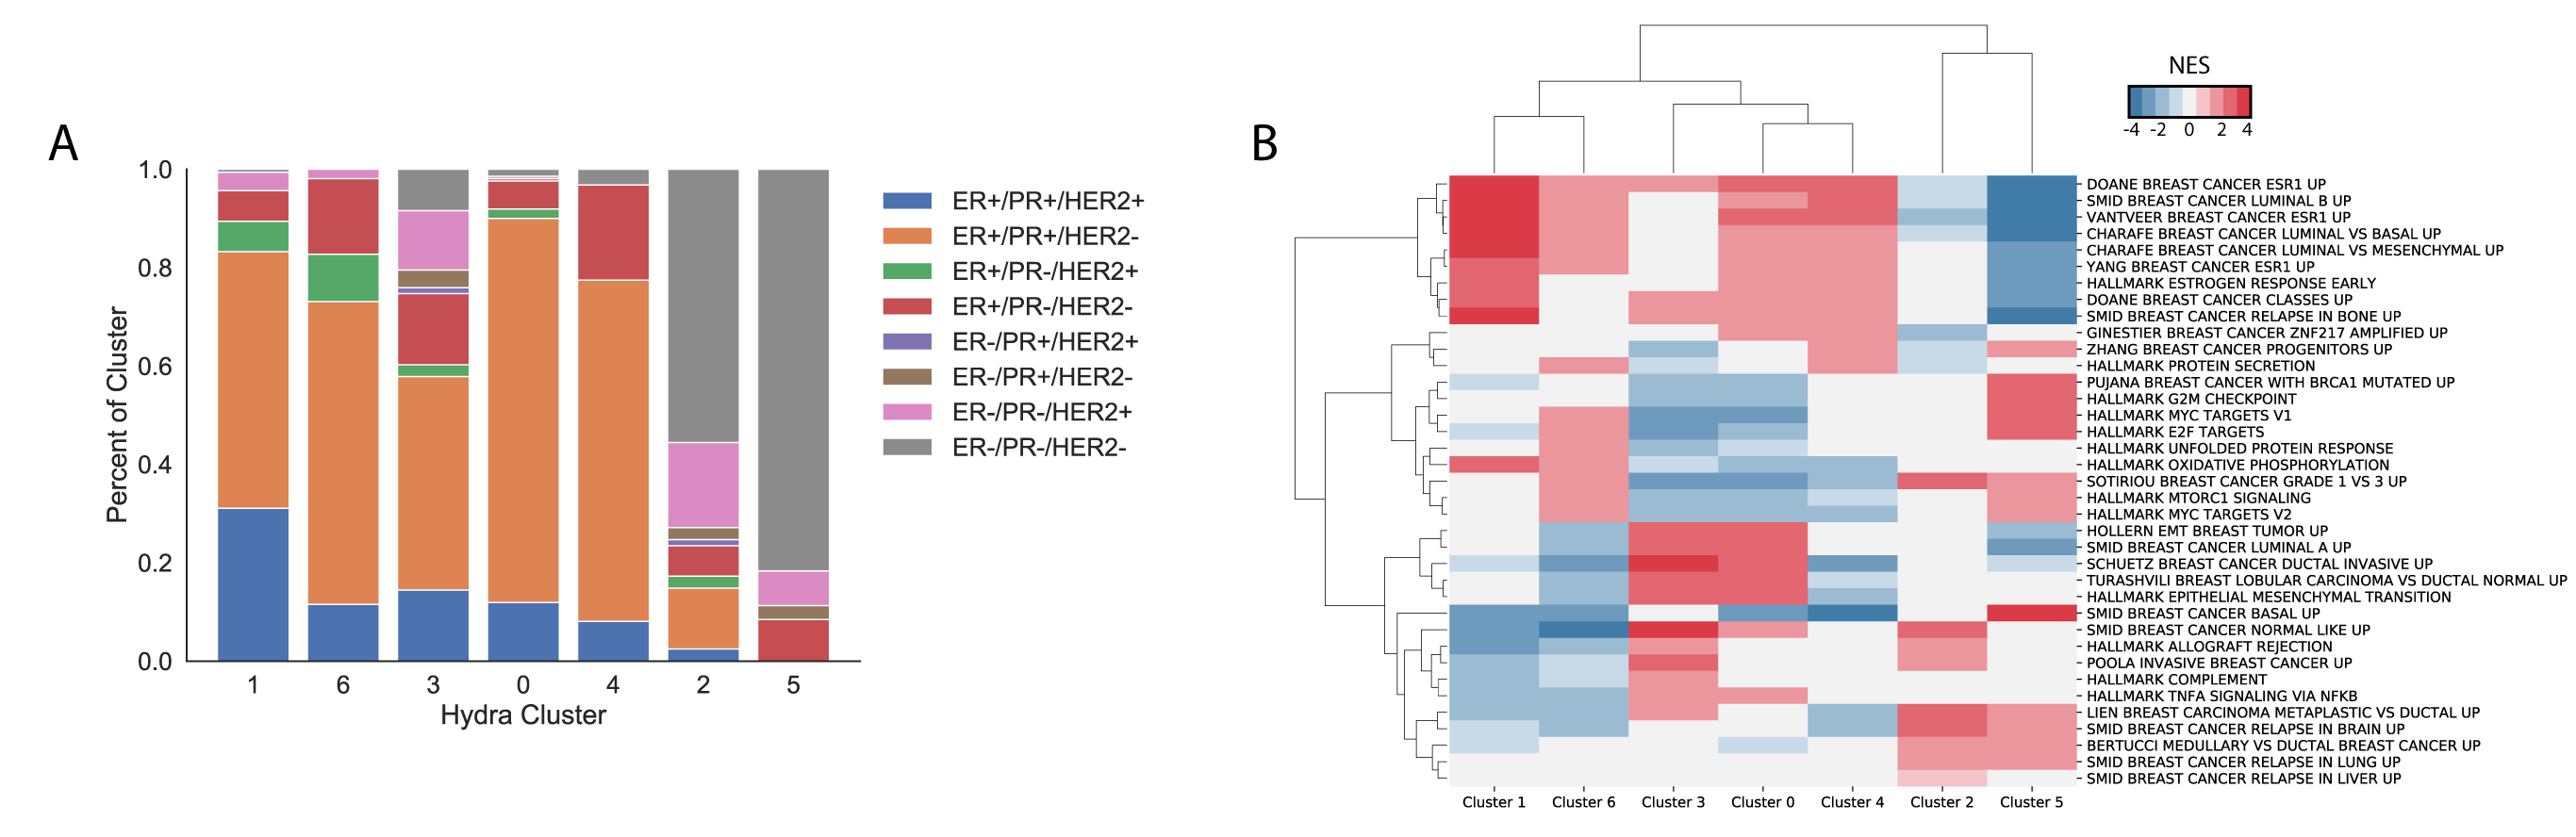
\includegraphics[width=1.1\linewidth]{images/tcga-brca-subtyping-figure@2x.png}
	\caption{Hydra Subtypes Identify Known Breast Cancer Subtypes.}
	\label{sfig:brca-subtypes}
\end{figure}


\begin{figure}
	\centering
	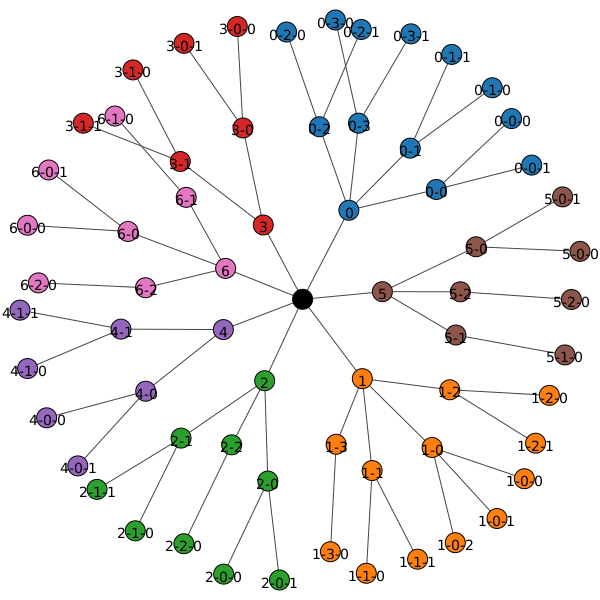
\includegraphics[width=0.8\linewidth]{images/tcga-brca-subcluster-tree.png}
	\caption{Iterative clustering reveals hidden structure within TCGA BRCA data. }
	\label{sfig:brca-ihydra}
\end{figure}

\begin{figure}
	\centering
	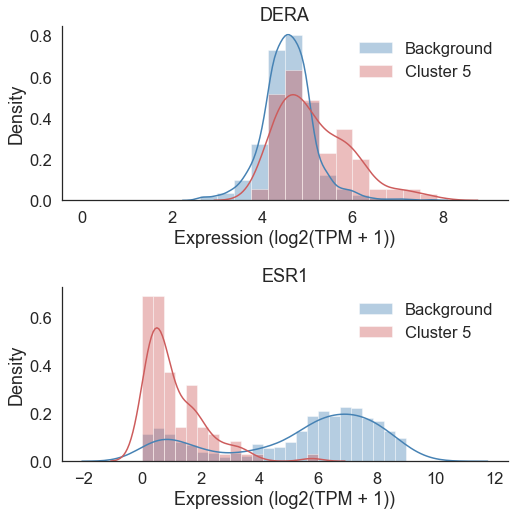
\includegraphics[width=0.75\linewidth]{images/example-subtyping-distribution-changes.png}
	\caption{Iterative clustering reveals hidden structure within TCGA BRCA data. }
	\label{sfig:brca-expression-subtypes}
\end{figure}


\begin{table}
\begin{tabular}{clcc}
	\toprule
	{} &                                         Gene Set &   NES & P-Value \\
	Cluster &                                                  &       &         \\
	\midrule
	0       &                SMID BREAST CANCER NORMAL LIKE UP &  3.08 &   0.002 \\
	0       &                  SMID BREAST CANCER LUMINAL A UP &  2.23 &   0.008 \\
	1       &                      SMID BREAST CANCER BASAL UP &  3.78 &   0.044 \\
	2       &                      SMID BREAST CANCER BASAL UP &  2.29 &   0.003 \\
	2       &               ZHANG BREAST CANCER PROGENITORS UP &  1.82 &   0.037 \\
	3       &                      DOANE BREAST CANCER ESR1 UP &  3.82 &   0.001 \\
	3       &                  SMID BREAST CANCER LUMINAL B UP &  3.19 &   0.001 \\
	3       &                   DOANE BREAST CANCER CLASSES UP &  3.12 &   0.001 \\
	3       &        CHARAFE BREAST CANCER LUMINAL VS BASAL UP &  3.09 &   0.001 \\
	3       &  CHARAFE BREAST CANCER LUMINAL VS MESENCHYMAL UP &  3.08 &   0.001 \\
	3       &            SMID BREAST CANCER RELAPSE IN BONE UP &  3.08 &   0.001 \\
	3       &                      SMID BREAST CANCER ERBB2 UP &  2.70 &   0.001 \\
	3       &                       YANG BREAST CANCER ESR1 UP &  2.61 &   0.001 \\
	3       &                   VANTVEER BREAST CANCER ESR1 UP &  2.49 &   0.001 \\
	3       &                  SMID BREAST CANCER LUMINAL A UP &  1.95 &   0.021 \\
	\bottomrule
\end{tabular}
	\caption{TCGA Triple Negative Breast Cancer Subtypes}
	\label{stab:tnbc-table}
\end{table}

\section*{Discussion}

The Discussion should be succinct and must not contain subheadings.

One of the benefits of this approach is that this provides a framework for understanding a population of patients and can identify subtypes that may benefit from future drug development. Investigation into subtype specific expression may also identify opportunities to repurpose available therapies for other diseases. This is particularly useful for pediatric cancer gene expression analysis where drug development has lagged and there is a need for novel therapies. 

One of the limitations of a non-parametric ranking approach to gene set enrichment is that it cannot account for the dynamic range in expression for a gene in a single-sample context. Therefore, we hypothesized that a GSEA method approach that does not account for this information will suffer if the background expression for a gene set is high. We see this in the HALLMARK Oxidative Phosphorylation analysis where the ssGSEA suffers from poor performance because the background expression is higher and thus is not well suited to identify subtle changes in expression.

ssGSEA method performed as well as the hydra method when the background expression is low, but the ssGSEA performance decreased when the baseline expression for a gene set is high. A larger effect size decreased the effect of baseline gene set expression. The hydra approach was not influenced by the baseline expression for a gene set.


\section*{Methods}

%Topical subheadings are allowed. Authors must ensure that their Methods section includes adequate experimental and characterization data necessary for others in the field to reproduce their work.

\subsection{Synthetic Data Generation}
A synthetic data analysis was done to assess the performance of the hydra mixture modeling approach compared to rank-based approaches. The synthetic data was generated from GTEx skeletal muscle data and the MSigDB hallmark gene sets \cite{consortium2013genotype,liberzon2011molecular}. We used the 26 Hallmark gene sets with at least 100 genes. We randomly assigned a subset of the samples to have over-expression for each gene set. This process was repeated twice to created synthetic training and test data. We compared the hydra method to single sample gene set enrichment analysis (ssGSEA) \cite{barbie2009systematic} and gene set variation analysis (GSVA) \cite{hanzelmann2013gsva}. Both methods are implemented in the GSVA package. These methods are used widely in the field and have been used to identify biological pathway activation and subtype tumors.

The MSigDB Hallmark gene sets were used to simulate biological pathway expression that reflects the gene set properties of a typical gene expression analysis \cite{liberzon2015molecular,liberzon2011molecular}. We also needed a large cohort of human tissue samples to infer differentially expressed genes. We used the GTEx skeletal muscle cohort \cite{consortium2013genotype}. To simulate subtype specific expression, we randomly sampled 25\% of the patient population and then we sampled from a normal distribution centered at 0.5 with a standard deviation of 0.5. We then added this value to 25\% of the genes in each Hallmark gene set to simulate coordinated expression of genes within a biological gene set.

We compared the predictive performance for identifying enriched genes using healthy tissue samples collected as part of the Genotype-Tissue Expression (GTEx) project \cite{lonsdale2013genotype}. The Molecular Signatures Database (MSigDB) provides a large set of curated gene lists for identifying biological functions for precision medicine applications. We used the Hallmark MSigDB gene sets to select genes with related biological functions and correlated expression \cite{liberzon2015molecular}. We then randomly sampled GTEx skeletal muscle samples, modified their expression values for a subset of the gene set genes. We did this process twice to generate synthetic training and test data. The same genes were used in the test and training data, but the values were sampled independently from a normal distribution at varying mean differences. 

We applied this analysis to all of the Hallmark gene sets, but we are showing two illustrative examples here (TODO: add figure ref). The Hallmark Glycolysis gene set includes 199 genes involved in glycolysis and gluconeogenesis. We sample 25\% of these genes to be differentially expressed and sampled a difference in expression value from a normal $\mathcal{N}(0.5, 0.5)$ or a $\mathcal{N}(1, 0.5)$. If this difference caused a negative expression value, then we set the expression value to be zero. The GTEx expression TPM values were generated using the Toil RNA-Seq pipeline \cite{vivian2017toil}. The reciever operator curves (ROC) were generated for the hydra, ssGSEA, and GSVA methods. The hydra method performed the best with an AUC (area under the curve) of X, but the ssGSEA method was comparable with an AUC of blank. The GSVA method performed the worst with an AUC of BLANK.



\bibliography{reference}

\section*{Acknowledgements (not compulsory)}

Acknowledgements should be brief, and should not include thanks to anonymous referees and editors, or effusive comments. Grant or contribution numbers may be acknowledged.

\section*{Author contributions statement}

J.P. conceived the analysis, conducted the analysis, and wrote the paper. O.M., H.B., S.S., and D.H. reviewed the results and contributed feedback. All authors reviewed the manuscript. 

\section*{Additional information}

To include, in this order: \textbf{Accession codes} (where applicable); \textbf{Competing financial interests} (mandatory statement). 

The corresponding author is responsible for submitting a \href{http://www.nature.com/srep/policies/index.html#competing}{competing financial interests statement} on behalf of all authors of the paper. This statement must be included in the submitted article file.

\beginsupplement
\section*{Supplementary Information}

\subsection*{Cancer Gene Expression Distributions are Multi-Modal}
\subsubsection*{Modes Correspond to Sex-Specific Expression}
Genes are expressed at different levels for different tissues. In addition to tissue specific expression, there are also biological features that influence gene expression across individuals. For example, age and gender are correlated with expression of some genes. A varying effects model where the mean and the effect of biological features change depending on the tissue can be used to make better predictions of gene expression. For example, a hierarchical model can identify sex-linked expression, but the current pan-cancer and pan-disease analyses are not able to detect sex-linked expression. An example of sex-linked expression that has been associated with cancer is the XIST gene \cite{yildirim2013xist}. XIST controls X-chromosome silencing in females and is not usually expressed in males (\figref{xist}). This is a clear example where assuming male and female gene expression comes from the same distribution leads to an exaggerated estimation of the outlier threshold. It is therefore difficult to identify potential cases where under-expression of XIST in females may contribute to their cancer. While the incidence of cancer is equal across boys and girls, boys tend to respond worse to therapy. An investigation into sex-linked gene expression may yield insights into the differences in response to cancer therapies for boys and girls. 

%%%%%%%%%%%%%%%
% XIST Figure %
%%%%%%%%%%%%%%%

\begin{figure}
\centering
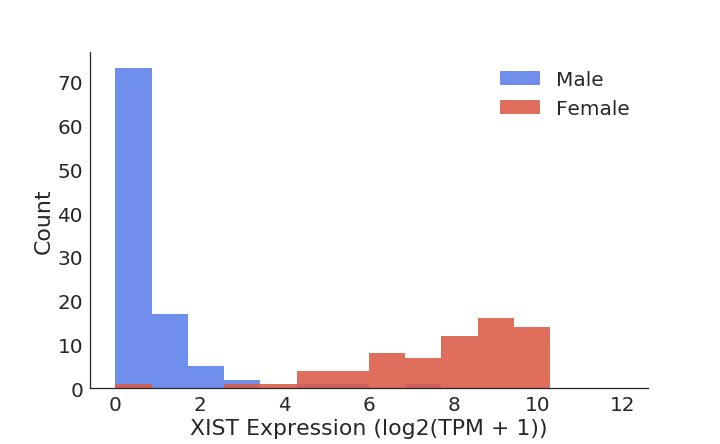
\includegraphics[width=0.75\linewidth]{images/xist-fig-2017-12-28.png}
\caption{Example of gender-specific expression that can be modeled in a hierarchical model. The XIST gene is involved in X chromosome silencing, so XIST is not expressed for males. XIST has been linked to cancer, but the Treehouse model overestimates the variance in XIST expression because females and males are modeled together. The proposed hierarchical model learns the differences between male and female XIST expression for improved model fit.}
\label{sfig:xist}
\end{figure}


%%%%%%%%%%%%%%%%%%%%%%%%%%
% MYCN Validation Figure %
%%%%%%%%%%%%%%%%%%%%%%%%%%

\begin{figure}
	\centering
	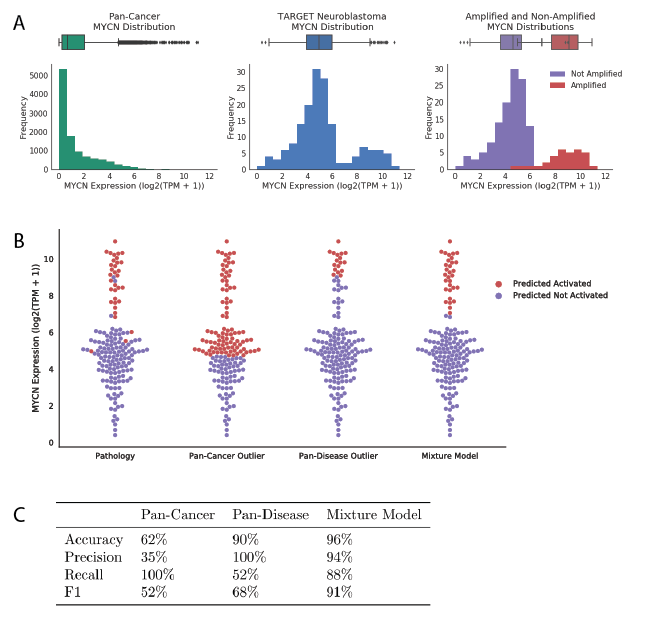
\includegraphics[width=0.75\linewidth]{images/MYCN-Figure.png}
	\caption{MYCN Validation}
	\label{sfig:mycn}
\end{figure}

%%%%%%%%%%%%%%%%%%%%%%%%%%%%%%%%
% Melanoma Gene Set Enrichment %
%%%%%%%%%%%%%%%%%%%%%%%%%%%%%%%%

\begin{figure}
	\centering
	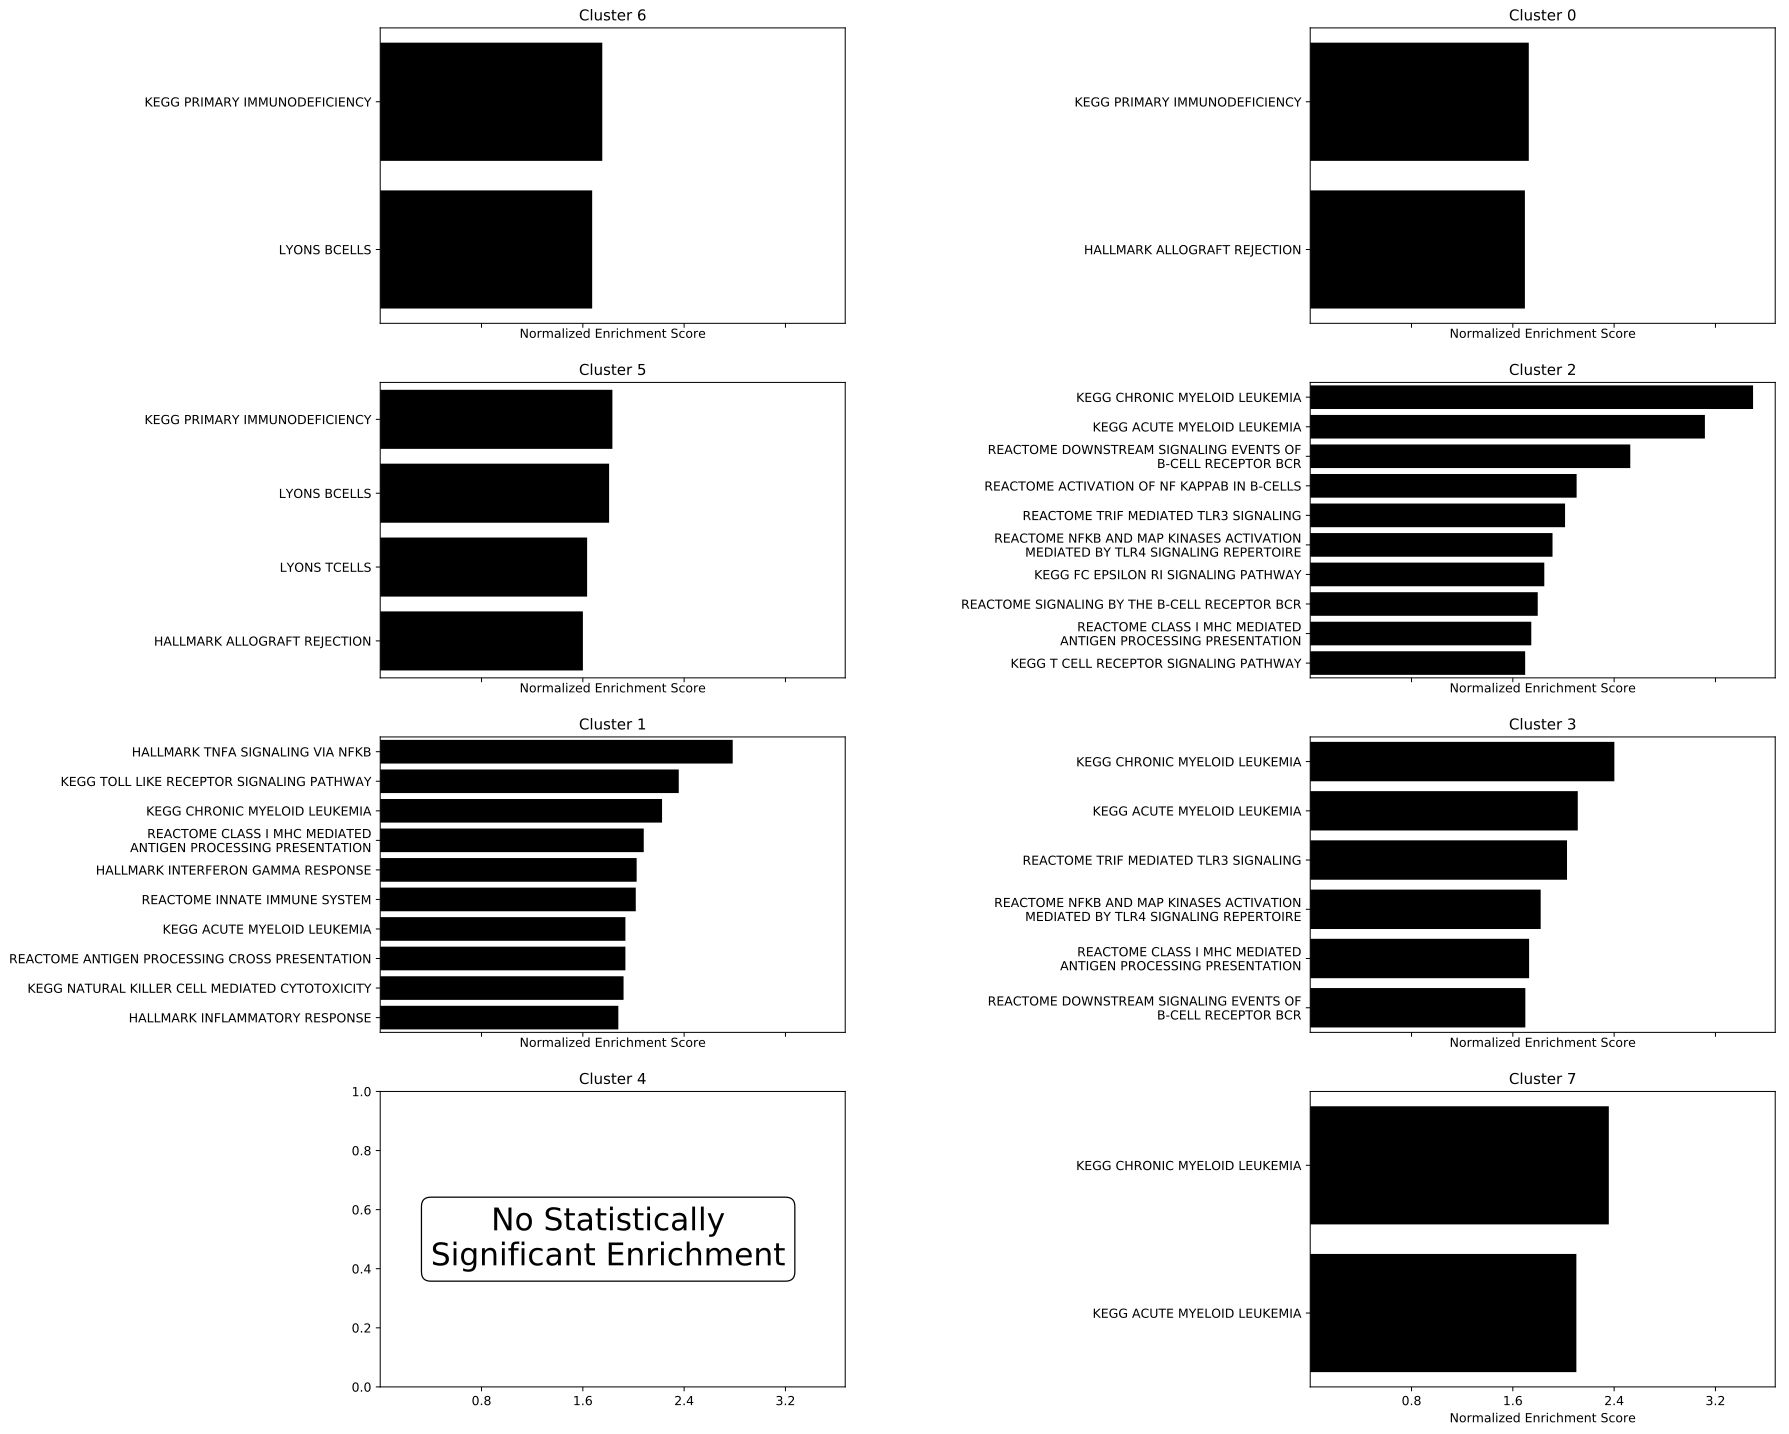
\includegraphics[width=0.75\linewidth]{images/melanoma-immune-subtype-enrichment.png}
	\caption{Melanoma Cluster Immune Gene Set Enrichment}
	\label{sfig:melanoma-gsea}
\end{figure}




\end{document}